%http://www.daniel-brettschneider.de/allgemein/latex-vorlage-fur-hausarbeiten-oder-abschlussarbeiten
\documentclass[12pt,a4paper,bibliography=totocnumbered,listof=totocnumbered, abstracton]{scrartcl}

\usepackage[autostyle=true,german=quotes]{csquotes}
\usepackage[utf8]{inputenc}
\usepackage{amsmath}
\usepackage{amsfonts}
\usepackage{amssymb}
\usepackage{amsthm}
\usepackage{graphicx}
\usepackage{fancyhdr}
\usepackage{tabularx}
\usepackage{geometry}
\usepackage{setspace}
\usepackage[right]{eurosym}
\usepackage[printonlyused]{acronym}
\usepackage{subfig}
\usepackage{floatflt}
\usepackage[usenames,dvipsnames]{color}
\usepackage{colortbl}
\usepackage{paralist}
\usepackage{array}
\usepackage{titlesec}
\usepackage{parskip}
\usepackage[right]{eurosym}
\usepackage[subfigure,titles]{tocloft}
\usepackage[pdfpagelabels=true]{hyperref}
\usepackage[ngerman]{babel}
\usepackage{booktabs}
\usepackage{listings}
\usepackage{csquotes}
\usepackage{siunitx}
\usepackage{tocloft}

\setlength{\cftfignumwidth}{2em}

\newtheoremstyle{Umgebung}	% name
{20pt}	% Space above, empty = `usual value'
{20pt} % Space below
{} % Body font
{} % Indent amount (empty = no indent, \parindent = para indent)
{\bfseries} % Thm head font
{} % Punctuation after thm head
{\newline} % Space after thm head: \newline = linebreak
{} % Thm head spec

\def\code#1{\texttt{#1}}
% "define" Scala
\lstdefinelanguage{scala}{
	morekeywords={abstract,case,catch,class,def,%
		do,else,extends,false,final,finally,%
		for,if,implicit,import,match,mixin,%
		new,null,object,override,package,%
		private,protected,requires,return,sealed,%
		super,this,throw,trait,true,try,%
		type,val,var,while,with,yield},
	otherkeywords={=>,<-,<\%,<:,>:,\#,@},
	sensitive=true,
	morecomment=[l]{//},
	morecomment=[n]{/*}{*/},
	morestring=[b]",
	morestring=[b]',
	morestring=[b]"""
}

\definecolor{dkgreen}{rgb}{0,0.6,0}
\definecolor{gray}{rgb}{0.5,0.5,0.5}
\definecolor{mauve}{rgb}{0.58,0,0.82}

\lstdefinestyle{myScalastyle}{
	frame=tb,
	language=scala,
	aboveskip=3mm,
	belowskip=3mm,
	showstringspaces=false,
	columns=flexible,
	basicstyle={\small\ttfamily},
	numbers=left,
	numberstyle=\tiny\color{gray},
	keywordstyle=\color{blue},
	commentstyle=\color{dkgreen},
	stringstyle=\color{mauve},
	frame=single,
	breaklines=true,
	breakatwhitespace=true,
	tabsize=2,
}


\theoremstyle{Umgebung}

\lstset{basicstyle=\footnotesize, captionpos=b, breaklines=true, showstringspaces=false, tabsize=2, frame=lines, numbers=left, numberstyle=\tiny, xleftmargin=2em, framexleftmargin=2em}
\makeatletter
\def\l@lstlisting#1#2{\@dottedtocline{1}{0em}{1em}{\hspace{1,5em} Lst. #1}{#2}}
\makeatother
\geometry{a4paper, top=27mm, left=30mm, right=20mm, bottom=35mm, headsep=10mm, footskip=12mm}
\hypersetup{unicode=false, pdftoolbar=true, pdfmenubar=true, pdffitwindow=false, pdfstartview={FitH},
	pdftitle={Ausarbeitung Projektvortrag Fuzzy-Regelung},
	pdfauthor={Joel Bartelheimer, Nico Müller},
	pdfsubject={Ausarbeitung Fuzzy-Reglung},
	pdfcreator={\LaTeX\ with package \flqq hyperref\frqq},
	pdfproducer={pdfTeX \the\pdftexversion.\pdftexrevision},
	pdfkeywords={Ausarbeitung Projektvortrag Fuzzy-Regelung},
	pdfnewwindow=true,
	colorlinks=true,linkcolor=black,citecolor=black,filecolor=magenta,urlcolor=black}
\pdfinfo{/CreationDate (D:20110620133321)}
\begin{document}
\titlespacing{\section}{0pt}{12pt plus 4pt minus 2pt}{-6pt plus 2pt minus 2pt}
% Kopf- und Fusszeile
\renewcommand{\sectionmark}[1]{\markright{#1}}
\renewcommand{\leftmark}{\rightmark}
\pagestyle{fancy}
\lhead{}
\chead{}
\rhead{\thesection\space\contentsname}
\lfoot{Ausarbeitung Projektvortrag Fuzzy-Regelung}
\cfoot{}
\rfoot{ Seite \thepage}
\renewcommand{\headrulewidth}{0.4pt}
\renewcommand{\footrulewidth}{0.4pt}
% Vorspann
\renewcommand{\thesection}{\Roman{section}}
\renewcommand{\theHsection}{\Roman{section}}
\pagenumbering{roman}
% ----------------------------------------------------------------------------------------------------------
% Titelseite
% ----------------------------------------------------------------------------------------------------------
\thispagestyle{empty}
\begin{center}
	
\includegraphics[width=5cm]{img/thm2.png}\\
	\vspace*{2cm}
	\Large
	\textbf{Fachbereich}\\
	\textbf{Mathematik, Naturwissenschaften und Informatik }\\
	\vspace*{2cm}
			\Huge
	\textbf{Ausarbeitung Projektvortrag Fuzzy-Regelung}\\
	\vspace*{1.5cm}
		\small
		\textbf{Im Rahmen der Veranstaltung:}\\
		\Large
	\textbf{Praktikum Künstliche Intelligenz(CS5330)}\\
	\vspace*{2cm}
	

	\normalsize
	\newcolumntype{x}[1]{>{\raggedleft\arraybackslash\hspace{0pt}}p{#1}}
	\begin{tabular}{x{7.5cm}x{7.5cm}}
		\rule{0mm}{5ex}\textbf{Autoren:} 
		\newline 
		\newline Joel Bartelheimer
		\newline joel.bartelheimer@mni.thm.de
		\newline 
		\newline Nico Müller
		\newline nico.mueller@mni.thm.de
		\newline
		& 
		\rule{0mm}{5ex}\textbf{Eingereicht bei:} 
		\newline
		\newline  Prof. Dr. Wolfgang Henrich
		\newline
		\newline\rule{0mm}{5ex}\textbf{Abgabedatum:} 
		\newline 24.04.2017
		\newline
	\end{tabular} 
\end{center}
\pagebreak

% ----------------------------------------------------------------------------------------------------------
% Verzeichnisse
% ----------------------------------------------------------------------------------------------------------
% TODO Typ vor Nummer
\renewcommand{\cfttabpresnum}{Tab. }
\renewcommand{\cftfigpresnum}{Abb. }
\settowidth{\cfttabnumwidth}{Abb. 10\quad}
\settowidth{\cftfignumwidth}{Abb. 10\quad}
\titlespacing{\section}{0pt}{12pt plus 4pt minus 2pt}{2pt plus 2pt minus 2pt}
\singlespacing
\rhead{INHALTSVERZEICHNIS}
\renewcommand{\contentsname}{II Inhaltsverzeichnis}
\phantomsection
\addcontentsline{toc}{section}{\texorpdfstring{II \hspace{0.35em}Inhaltsverzeichnis}{Inhaltsverzeichnis}}
\addtocounter{section}{1}
\tableofcontents
\pagebreak
\listoffigures
\pagebreak
\listoftables
\pagebreak
\renewcommand{\lstlistlistingname}{Listingverzeichnis}
\lstlistoflistings
\pagebreak
\rhead{VERZEICHNISSE}


% ----------------------------------------------------------------------------------------------------------
% Inhalt
% ----------------------------------------------------------------------------------------------------------
% Abstände Überschrift
\titlespacing{\section}{0pt}{12pt plus 4pt minus 2pt}{-6pt plus 2pt minus 2pt}
\titlespacing{\subsection}{0pt}{12pt plus 4pt minus 2pt}{-6pt plus 2pt minus 2pt}
\titlespacing{\subsubsection}{0pt}{12pt plus 4pt minus 2pt}{-6pt plus 2pt minus 2pt}
% Kopfzeile
\renewcommand{\sectionmark}[1]{\markright{#1}}
\renewcommand{\subsectionmark}[1]{}
\renewcommand{\subsubsectionmark}[1]{}
\lhead{Kapitel \thesection}
\rhead{\rightmark}
\onehalfspacing
\renewcommand{\thesection}{\arabic{section}}
\renewcommand{\theHsection}{\arabic{section}}
\setcounter{section}{0}
\pagenumbering{arabic}
\setcounter{page}{1}

\newtheorem{bsp}{Beispiel}
\newtheorem{defnt}{Definition}

% ----------------------------------------------------------------------------------------------------------
% Einleitung
% ----------------------------------------------------------------------------------------------------------
\begin{abstract} 
	Die vorliegende Hausarbeit bearbeitet eine Problemstellung des autonomen Fahrens. Konkret soll ein durch einen Fuzzy-Regler gesteuertes Autos einem anderen Auto im optimalen Abstand folgen. Zunächst werden die physikalischen Bedingungen für die beiden Autos erläutert. Anschließen wird darauf eingegangen wie man mit Hilfe von numerischer Integration die tatsächliche Geschwindigkeit bzw. Bewegung eines Fahrzeugs simulieren kann. Der eigentlich Fuzzy-Regler wurde mithilfe von funktionaler Programmierung implementiert. Zuletzt wird die GUI sowie das Zusammenspiel zwischen den Modellen und der GUI vorgestellt.

\end{abstract} 
\newpage

\section{Problemstellung}

Die gestellte Aufgabe zur praktischen Ausarbeitung kommt aus dem Themengebiet des autonomen Fahrens. Es soll ein Fuzzy-Regler eingesetzt werden um ein Fahrzeug so zu steuern, dass es einem anderen, durch den Menschen gesteuerten, Fahrzeug folgt.  Hierbei ist zu beachten, dass hier bei nur die Geschwindigkeit bzw. Bewegung in einer Achse kontrolliert wird. Das bedeutet, dass nur das Gas- sowie das Bremspedal jedoch nicht das Lenkrad geregelt werden muss. Außerdem gehen wir davon aus, dass es sich bei dem gesteuerten Fahrzeug um ein Fahrzeug mit Automatikgetriebe handelt und somit das Kuppeln sowie das Schalten der Gänge ebenfalls irrelevant ist. 

Bei der Implementierung sollte darauf geachtet werden, dass beide Fahrzeuge, so weit wir möglich, den physikalischen Gesetzen unterliegen. Dies bedeutet, dass z.B. die Fahrwiderstände wie Luftwiderstand, Rollwiderstand usw. beachtet werden müssen. Ebenfalls sollten beide Fahrzeuge durch eine physikalische Spezifikation, wie z.B. das Gewicht, definiert werden. Beide Fahrzeuge sollten hierbei der gleichen physikalische Spezifikation unterliegen, um keines der beiden Fahrzeuge einen Vorteil zu bieten.

\begin{figure}
	\centering
	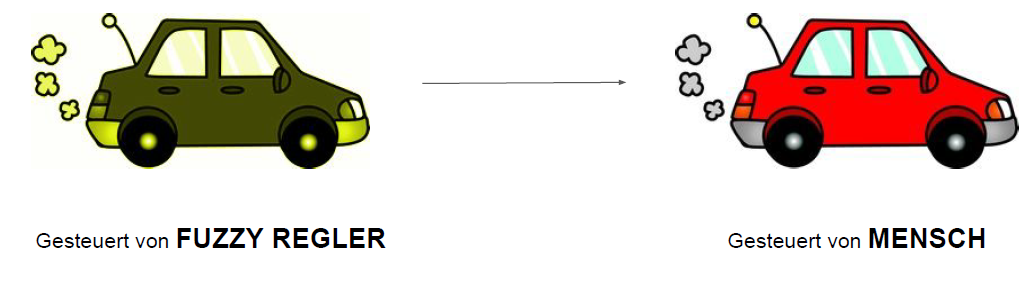
\includegraphics[width=0.9\linewidth]{img/practical/problem}
	\caption{Problemstellung}
	\label{fig:problem}
\end{figure}

\section{Implementierung}

In diesem Kapitel wird eine Lösung für das gestellte Problem vorgestellt. Wir empfehlen dem Leser zuerst die Ausarbeitung zum theoretischen Teil der Fuzzy-Regelung zu lesen, da hier keine Grundlagen erläutert werden.

\subsection{Funktionale Programmierung}

Als funktionale Programmierung bezeichnet man ein Programmierparadigma in dem alle Programme lediglich aus Funktionen bestehen. Hierbei können neue Funktionen aus bereits bestehenden Funktionen zusammengesetzt werden. Ebenfalls werden Funktionen in der funktionalen Programmierung als Wert angesehen. Dies erlaubt es Funktionen als Parameter oder Rückgabe zu verwenden, dies nennt man \enquote{Funktion höhrer Ordnung}. In sogenannten \enquote{reinen} funktionalen Programmiersprachen gibt es keine Variablen womit Seiteneffekte vollkommen ausgeschlossen werden. Für unsere Implementierung wird die Sprache Scala\footnote{https://www.scala-lang.org/} verwendet. Scala ist eine JVM-Sprache die funktionale Programmierung und Objektorientierte Programmierung verbindet. Wir haben diese Sprache gewählt, da wir einerseits unsere Kenntnisse in der Sprache durch das Projekt erweitern wollten aber anderseits auch der Meinung waren, dass sich eine Fuzzy-Regelung einfacher mithilfe von Funktionen höherer Ordnung ausdrücken lässt.

\subsubsection{Map, Reduce, Filter}

Die drei Funktionen map, filter und fold sind essentiell um die funktionale Programmierung zu verstehen. \code{map} wendet eine Funktion auf jedes Element einer Liste an und kreiert somit eine neue Liste (siehe Abbildung \ref{fig:map}). Die Funktion \code{filter} entfernt genau die Element einer List, die eine mit einer Funktion verbunden ein boolesches \code{false} liefern (siehe Abbildung \ref{fig:filter}). Die Funktion \code{fold} oder auch \code{reduce} wendet eine Funktion mit zwei Parametern solange auf Paare der Liste an, bis nur noch ein Element in der Liste enthalten ist (siehe Abbildung \ref{fig:reduce}).

\begin{figure}
	\centering
	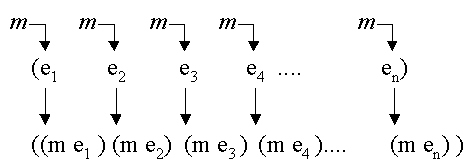
\includegraphics[width=0.6\linewidth]{img/practical/map}
	\caption{Veranschaulichung Map Funktion}
	\label{fig:map}
\end{figure}

\begin{figure}
	\centering
	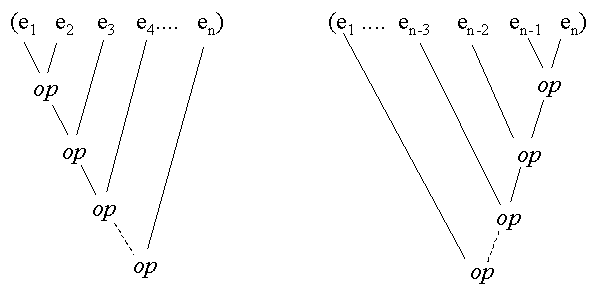
\includegraphics[width=0.6\linewidth]{img/practical/reduction}
	\caption{Veranschaulichung Reduce Funktion}
	\label{fig:reduce}
\end{figure}

\begin{figure}
	\centering
	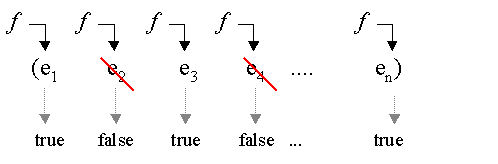
\includegraphics[width=0.6\linewidth]{img/practical/filter}
	\caption{Veranschaulichung Filter Funktion}
	\label{fig:filter}
\end{figure}

\subsection{Modell des Fahrzeugs}

Die Modelle der beiden Fahrzeuge werden in der Klasse \enquote{Car} realisiert (siehe Abbildung \ref{fig:car}). Jedes erstellte Fahrzeug hat ein vorgegebenes Gewicht in $kg$, ein Strömungswiderstandskoeffizient (dimensionslos) sowie eine gegebene Fläche der projizierte Stirnfläche in $m^2$. Ebenfalls wird eine maximale Brems bzw. Antriebskraft festgelegt. Wir haben für unser Modell diese Werte von realen Fahrzeugen übernommen und uns auf die Werte aus Tabelle \ref{table:car} festgelegt.

Zusätzlich wird für jedes Objekt des Typs \enquote{Car} die aktuelle Position relativ zum Null Punkt in $m$, die aktuelle Geschwindigkeit in $m/s$ sowie  die aktuelle Beschleunigung in $m/s^2$ dokumentiert. Der Nutzer der Klasse hat die Möglichkeit die Brems bzw. Antriebskraft in $N$ für das Auto über ein Interface zu setzen.

\begin{figure}
	\centering
	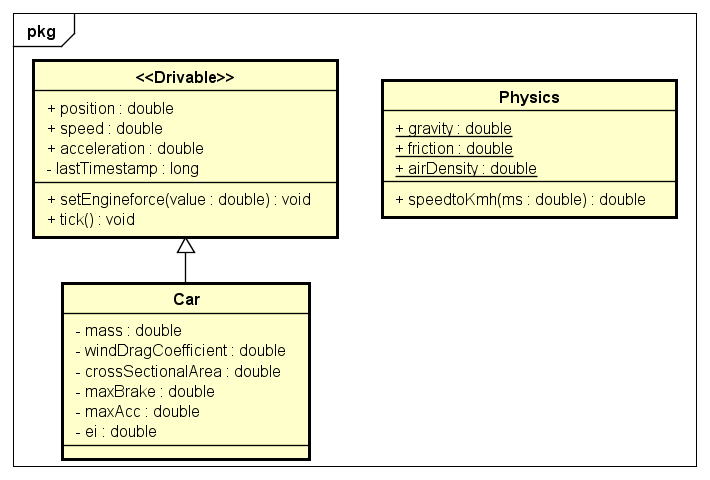
\includegraphics[width=0.7\linewidth]{img/practical/car-diagram}
	\caption{UML der Klasse Auto und deren Nachbarklassen.}
	\label{fig:car}
\end{figure}

% Please add the following required packages to your document preamble:
% \usepackage{booktabs}
\begin{table}[]
	\centering
	\caption{Physikalische Spezifikation der Fahrzeuge}
	\label{table:car}
	\begin{tabular}{@{}llll@{}}
		\toprule
		Eigenschaft                     & Wert & Einheit & Bezeichner           \\ \midrule
		Gewicht                         & 1540 & $kG$    & $m_{Fzg}$            \\
		Zuladung                        & 0    & $kG$    & $m_{Zu}$             \\
		Strömungswiderstandskoeffizient & 0.67 & -       & $cw$                 \\
		Projizierte Stirnfläche         & 1.86 & $m^2$   & $A$                  \\
		Maximale Bremskraft             & 8000 & $N$     & $\overline{F}_{max}$ \\
		Maximale Antriebskraft          & 3000 & $N$     & $ {F}_{max} $        \\
		Massefaktor                     & 1    & -       & $ {e}_{i} $          \\ \bottomrule
	\end{tabular}
\end{table}


\begin{table}[]
	\centering
	\caption{Physikalische Spezifikation der Umwelt}
	\label{table:physics}
	\begin{tabular}{@{}llll@{}}
		\toprule
		Eigenschaft                     & Wert & Einheit & Bezeichner           \\ \midrule
		Erdanziehungskraft	            & 9,81 & $m/s^2$    & $g$            \\
		Zuladung                        & 1.2  & $kG/m^3$   & $p_{Luft}$             \\
		Strömungswiderstandskoeffizient & 0.01 & -       & $f_{roll}$                 \\ \bottomrule       
	\end{tabular}
\end{table}

\subsubsection{Bestimmung der Beschleunigung}

Um die gesetzte Brems bzw. Antriebskraft, unter Berücksichtigung der physikalischen Gesetze, in eine Beschleunigung umzurechnen, betrachten wir zunächst die Fahrwiderstände die ein Fahrzeug überwinden muss. Als Fahrwiderstand $F_{FW}$ wird die Summe der Widerstände bezeichnet, die ein Fahrzeug mit Hilfe einer Antriebskraft überwinden muss, um das Fahrzeug zu bewegen. Dazu gehört der Luftwiderstand $F_{Luft}$, der Rollwiderstand $F_{Roll}$, der Steigungswiderstand $F_{Steig}$ sowie der Beschleunigungswiderstand $F_{B}$.

\paragraph{Luftwiderstand}

Der Luftwiderstand ist maßgeblich für die Höchstgeschwindigkeit eines Fahrzeugs. Er hängt von der aerodynamischen Form des Fahrzeuges ab und steigt mit der Geschwindigkeit ins Quadrat. Außerdem spielt die momentane Luftdichte $p_{Luft}$ in $kg/m^3$ eine Rolle für den Luftwiderstand. Diese ist abhängig von der Höhe in der Atmosphäre sowie der Temperatur der Atmosphäre.  Wir haben für diese Umgebungsvariable einen Wert von $1,2$ gewählt, dies entspricht der Luftdichte bei einer Temperatur von $20^\circ\text{C}$ auf Höhe des Meeresspiegels.

\begin{figure}
	\centering
	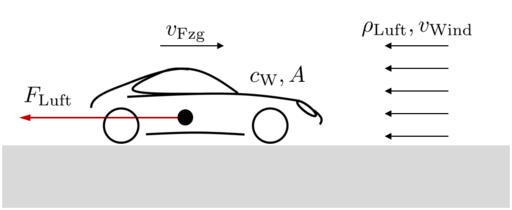
\includegraphics[width=0.7\linewidth]{img/practical/Luftwiderstand}
	\caption{Prinzipskizze zum Luftwiderstand an Fahrzeugen (Simon Herzog (https://commons.wikimedia.org/wiki/File:Luftwiderstand.png)}
	\label{fig:luftwiderstand}
\end{figure}

\begin{equation}
F_{Luft} = cw \cdot A \cdot \frac{p_{Luft} \cdot v_{Fzg}^2}{2}
\end{equation}

\paragraph{Rollwiderstand}

Der Rollwiderstand beschreibt die nötige Arbeit um einen Reifen auf einer Kontaktfläche zu rollen. Durch die Fahrzeugmaße und das elastische Material des Reifens sowie dem Boden werden diese zusammengedrückt und bilden keine optimale Kreisform mehr. Diese Eigenschaft wird durch den Rollwiderstandskoeffizient $f_{Roll}$ abstrahiert. Wir haben für diese Umgebungsvariable einen Wert von $0,01$ gewählt was einem Autoreifen auf einem Asphaltboden entspricht. In die Formel spielt außerdem die Erdbeschleunigung $g$ sowie der Steigungswinkel  $a$ eine Rolle. Wenn der Steigungswinkel steigt oder sinkt, also $ |a|  \gg 0$, konvergiert der Rollwiderstand gegen $0$. 

\begin{figure}
	\centering
	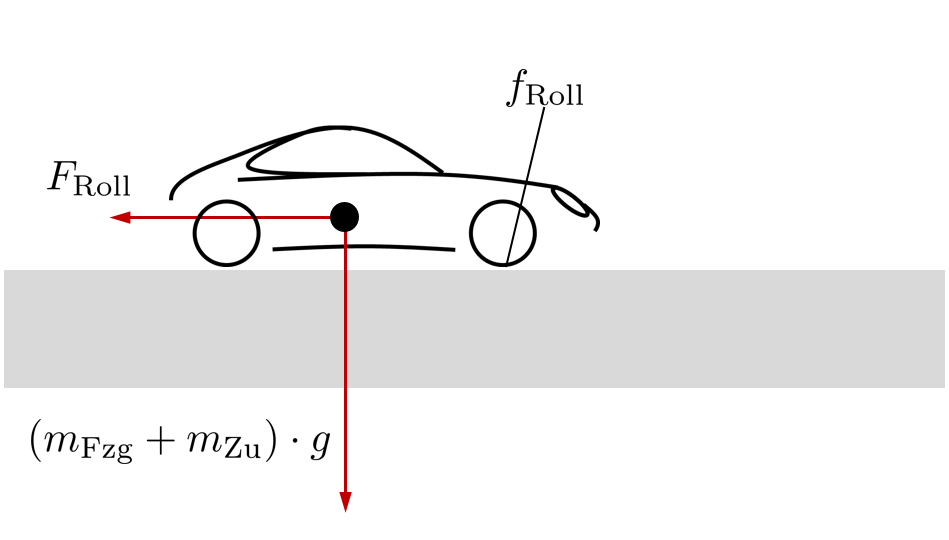
\includegraphics[width=0.7\linewidth]{img/practical/Rollwiderstand}
	\caption{Prinzipskizze zum Rollwiderstand an Fahrzeugen (Simon Herzog (https://commons.wikimedia.org/wiki/File:Rollwiderstand.png)}
	\label{fig:Rollwiderstand}
\end{figure}

\begin{equation}
F_{Roll} = f_{Roll} \cdot (m_{Fzg} + m_{Zu}) \cdot g \cdot cos(a)
\end{equation}


\paragraph{Steigungswiderstand}

Der Steigungswiderstand beschreibt die nötige Kraft die benötigt wird um die Maße des Fahrzeugs über die Steigung zu bewegen. Falls die Steigung negativ ist, wird der Steigungswiderstand negativ und beeinflusst somit das Fahrzeug positiv. Der Steigungswiderstand spielt in unserer Aufgabenstellung z.Z. keine Rolle, da von einer ebenen Strecke ausgegangen werden soll. Dennoch wurde dieser im Sinne der Vollständigkeit implementiert und hier aufgeführt.

\begin{figure}
	\centering
	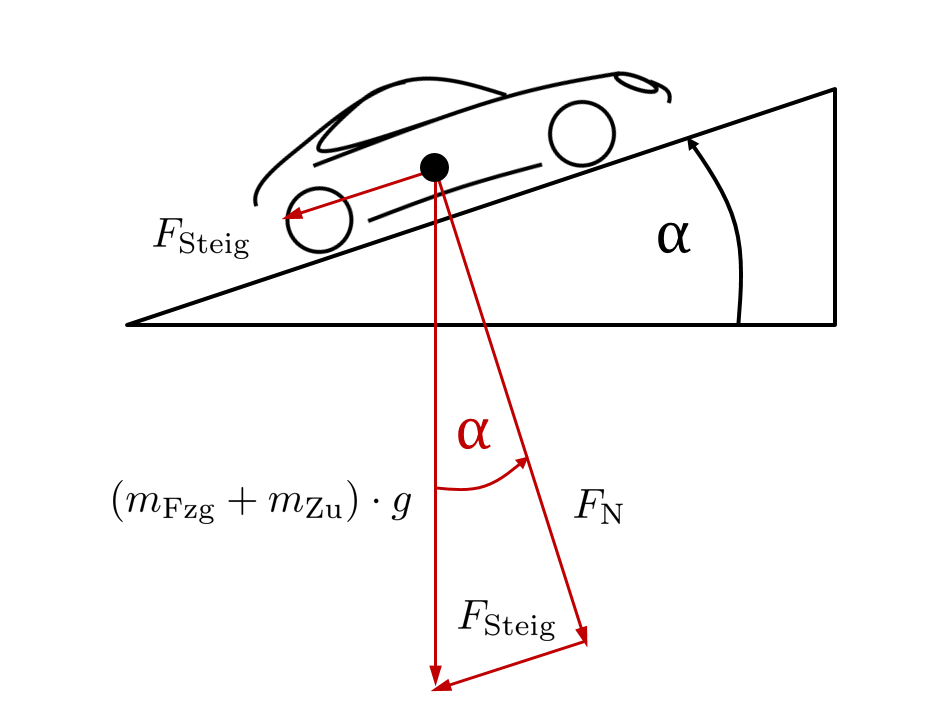
\includegraphics[width=0.7\linewidth]{img/practical/Steigungswiderstand}
	\caption{Prinzipskizze zum Steigungswiderstand an Fahrzeugen (Simon Herzog (https://commons.wikimedia.org/wiki/File:Steigungswiderstand.png)}
	\label{fig:Steigungswiderstand}
\end{figure}

\begin{equation}
F_{Steig} = (m_{Fzg} + m_{Zu}) \cdot g \cdot sin(a)
\end{equation}

\paragraph{Beschleunigungswiderstand}

Der Beschleunigungswiderstand beschreibt die nötige Kraft die benötigt wird um die Beschleunigung eines Fahrzeugs zu ändern. Dieser Widerstand entsteht durch die Trägheit des Fahrzeugs. Der Massefaktor $e_i$ ($\ge 1$) fasst den translatorischer Anteil, also Maße die sich in Fahrtrichtung bewegt sowie den rotatorischer Anteil, also alle rotierende Teile im Antriebsstrang (Motor, Kurbelwelle, Kupplung, Räder) zusammen. Der Massefaktor ist somit auch stark abhängig vom gewählten Gang des Fahrzeugs. In unserem Modell ist der Massefaktor auf 1 gesetzt.

\begin{figure}
	\centering
	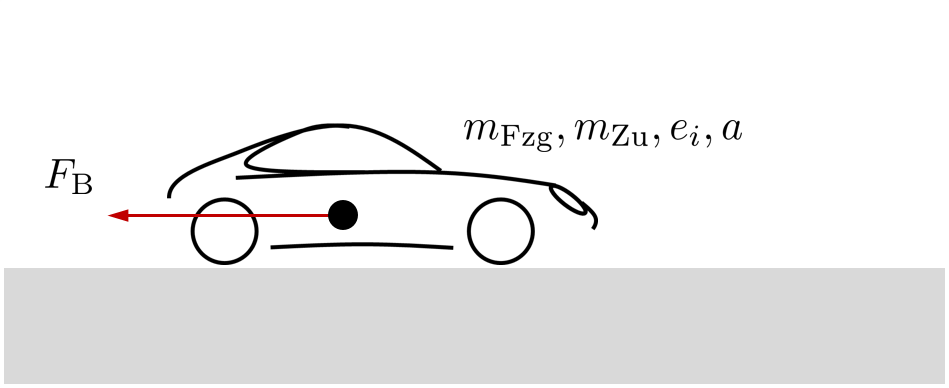
\includegraphics[width=0.7\linewidth]{img/practical/Beschleunigungswiderstand}
	\caption{Prinzipskizze zum Beschleunigungswiderstand an Fahrzeugen (Simon Herzog (https://commons.wikimedia.org/wiki/File:Beschleunigungswiderstand.png)}
	\label{fig:Beschleunigungswiderstand}
\end{figure}

\begin{equation}
 F_{B}=(e_{i}\cdot m_{Fzg} +m_{Zu}) \cdot a
\end{equation}

\begin{equation}
F_{FW} = F_{Luft} + F_{Roll} + F_{Steig} + F_{B}
\end{equation}

Um nun die tatsächliche Kraft zu erhalten müssen die Fahrwiderstände von der Antriebskraft subtrahiert werden. Dieser Kraft, definiert als $kg * m/s^2$, kann nun in die aktuelle Beschleunigung umgerechnet werden.

\begin{equation}
a = \frac{F - F_{FW}}{m_{Fzg} + m_{Zu}}
\end{equation}

\subsubsection{Bestimmung der Position}

Die Position eines jeden Fahrzeugs lässt sich über die Integration der Beschleunigung errechnen. Durch Ableitung der Position (siehe Gl. 1) ergibt sich die Geschwindigkeit (siehe Gl. 2). Durch ein weiteres Ableiten erhält man die Beschleunigung (siehe Gl. 3). Da unser System zunächst nur die Beschleunigung bereitsteht, lässt sich durch die Integration auf die Geschwindigkeit (siehe Gl. 4) sowie in einem weiteren Schritt auf die Position schließen (siehe Gl. 5).

\begin{equation}
	s(t) = \text{Position zur Zeit t}
\end{equation}

\begin{equation}
	\dot{s}(t) = v(t) = \text{Geschwindigkeit zur Zeit t}
\end{equation}

\begin{equation}
	\ddot{s}(t) = \dot{v}(t) = a(t) = \text{Beschleinung zur Zeit t}
\end{equation}

\begin{equation}
	\begin{aligned}
		\dot{v}(t)                 & = a(t)                        \\
		\int_{0}^{t} \dot{v}(t) dt & = \int_{0}^{t} a(t) dt        \\
		v(t)\Big|_0^t              & = a(t) \cdot t \Big|_0^t      \\
		v(t) - v(0)                & = a(t) \cdot t - a(0) \cdot 0 \\
		v(t)                       & = a(t) \cdot t + v(0)
	\end{aligned}
\end{equation}

\begin{equation}
\begin{aligned}
	\dot{s}(t)                 & = v(t)                                              \\
	\int_{0}^{t} \dot{s}(t) dt & = \int_{0}^{t} v(t) dt                              \\
	\int_{0}^{t} \dot{s}(t) dt & = \int_{0}^{t} a(t) \cdot t + v(0) dt               \\
	s(t)\Big|_0^t              & = 0,5 \cdot a(t) \cdot t^2 + v(t) \cdot t \Big|_0^t \\
	s(t) - s(0)                & = 0,5 \cdot a(t) \cdot t^2 + v(t) \cdot t           \\
	s(t)                       & = 0,5 \cdot a(t) \cdot t^2 + v(t) \cdot t + s(0)
\end{aligned}
\end{equation}

\paragraph{Numerische Integration}

Die numerische Integration in unserem System wird durch eine kontinuierliche, schrittweise Integration umgesetzt. Hierfür muss in zyklischen Abständen die Beschleunigung gemessen werden und dann die draus resultierende Geschwindigkeit und Position berechnet und aktualisiert werden. Wichtig ist hierbei, dass die Zeit zwischen diesen zyklischen Aufrufen festgehalten wird.

Im Code Beispiel (siehe Listing \ref{lst:integration}) wird in der Funktion \code{tick()} die numerische Integration implementiert. Die Variable \code{past} enthält einen Zeitstempel der gespeichert wurde, als die Funktion das letzte mal aufgerufen wurde. Wichtig ist hierbei, dass der Sichtbarkeitsbereich der Variablen außerhalb der Funktion liegt. So kann bei jedem Aufruf die vergangene Zeit zwischen dem aktuellen und vorherigen Aufruf bestimmt werden. Nach Abschluss der Berechnung wird Zeitstempel überschrieben.

\begin{lstlisting}[style=myScalastyle, caption=Numerische Integration, label=lst:integration]]
	var acceleration: Double = 0
	var speed: Double = 0
	var position: Double = 0
	var past: Long = System.currentTimeMillis()

	def tick(): Unit = {
		// Bestimmen der aktuellen Zeit
		val now = System.currentTimeMillis()
		// Berechnung der vergangenen Zeit in Sekunden
		val t: Double = (now - past) / 1000.0 
		
		// Erste Schritt der Integration
		acceleration = (engineForce - antiForce) / mass
		// Zweiter Schritt der Integration
		speed += (acceleration * t)
		// Dritter Schritt der Integration
		position += ((0.5 * acceleration * t * t) + speed * t)

		// Speichern der Aufrufszeit
		past = now;
	}
\end{lstlisting}

\subsection{Modell der Wissensbasis}

Die Wissensbasis besteht aus der Regelbasis und der Datenbasis. Alle Wertebereiche für die Eingangsgrößen und Stellgrößen sowie die dazugehörigen linguistischen Termen und dazu assoziierten Fuzzy-Mengen gehören zu der Datenbasis. Die Regelbasis besteht aus den linguistischen Kontrollregeln. Die Wissensbasis soll durch den Benutzer zur Laufzeit des Programms konfigurierbar sein. Aus diesem Grund wurden alle nötigen Parameter in ein Konfigurationsobjekt \code{FuzzyConfig} gebettet das zur jeder Zeit vom Fuzzy-Regler geladen werden kann. Um das Verständnis zu verbessern werden nun die einzelnen Komponenten der Wissensbasis und deren dazugehörigen Modellierungen vorgestellt.

\paragraph{Eingangs- Ausgangsgrößen}

Für jede messbare Eingangsgröße und jede Ausgangsgröße muss ein Wertebereich und ein Bezeichner festgelegt werden, sodass andere Programmteile diese wieder erkennen können. Diese Größen nennen wir \code{FuzzyValueConnector}.

\begin{figure}
	\centering
	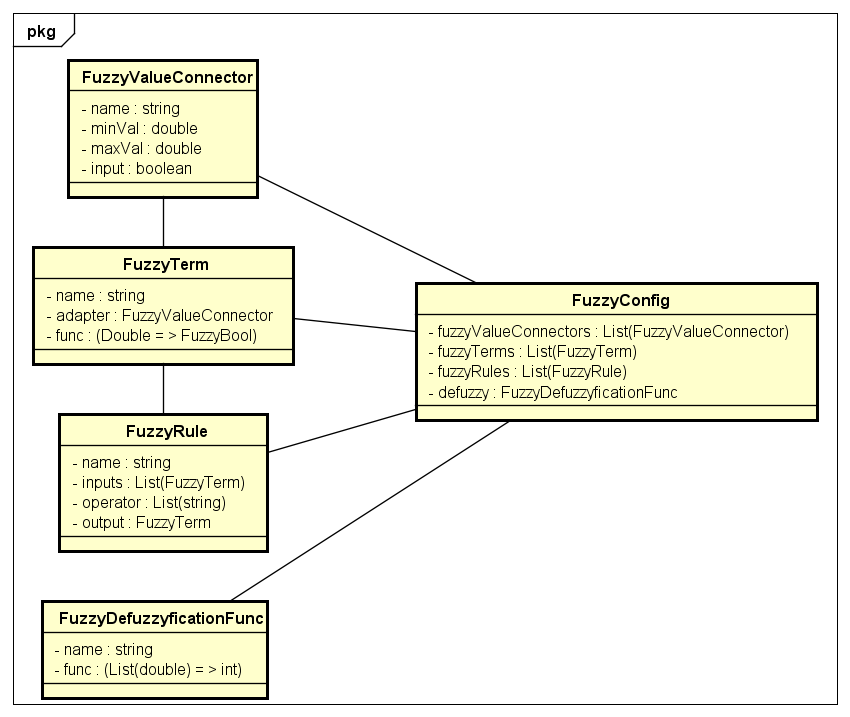
\includegraphics[width=0.7\linewidth]{img/practical/valueconnector}
	\caption{Modellierung der Wissensbasis}
	\label{fig:valueconnector}
\end{figure}

\paragraph{Fuzzy-Menge und Linguistischer Term}

Da ein linguistischer Term immer nur einer Fuzzy-Menge zugeordnet sein sollte, wurden diese Elemente in unserem Model zusammen in der Klasse \code{FuzzyTerm} implementiert. Die eigentliche Zugehörigkeitsfunktion wird durch die Funktion höherer Ordnung \code{(Double => FuzzyBool)} ausgedrückt. Wobei \code{FuzzyBool} nur ein Fließkommazahl in den Grenzen $\left[0,1\right]$ ist.

\paragraph{Fuzzy-Regeln}

Die Regelbasis in Form von linguistischen "Wenn - Dann - Regeln" wird durch die Klasse \code{FuzzyRule} modelliert. Jede Regel wird durch ihren Namen identifiziert und enthält eine List von \code{FuzzyTerm} die die Eingangsgrößen darstellen. Die Verknüpfung dieser Eingangsgrößen wird durch eine Liste von Operatoren modelliert. Außerdem wird eine Ausgangsgröße, ebenfalls in Form eines \code{FuzzyTerm} festgelegt.

\paragraph{Defuzzyfizierungs-Methoden}

Die Aufgabe der Defuzzyfizierungs-Methoden ist es aus der Ausgangsfuzzymenge einen Stellwert auszuwählen. In unserer Modellierung arbeitet die Defuzzyfizierungs-Methoden mit einer Liste aller im Wertebereich enthaltenen Werte auf die die kombinierten Zugehörigkeitsfunktion aller Regeln bereits angewendet wurden. Sie liefert dann einen Stellwert in diesem Wertebereich zurück. Die Defuzzyfizierungs-Methoden wird durch die Funktion höherer Ordnung \code{List[Double] => Int)} beschrieben und durch einen Namen identifiziert und in der Klasse \code{FuzzyDefuzzyficationFunc} zusammengefasst.

\subsection{Modell des Fuzzy-Reglers}

Die eigentliche Fuzzy-Regelung findet in der Klasse \code{FuzzyCarController} statt. Die Klasse wird mit einer \code{FuzzyConfig} und zwei Objekten des Interfaces \code{Drivable} erzeugt. Eine Instanz stellt hierbei das Verfolger- und eins das Vorausfahrende Fahrzeug dar. Es wird eine Funktion \code{tick()} bereitgestellt. Diese muss vom Nutzer der Klasse zyklisch aufgerufen werden um einen Berechnungsschritt auszuführen. Jeder Berechnungsschritt durchläuft vier Phasen.

\begin{figure}
	\centering
	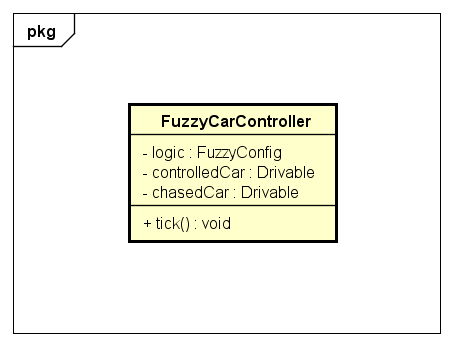
\includegraphics[width=0.4\linewidth]{img/practical/controller-diagram}
	\caption{Interfaces des Fuzzy-Reglers}
	\label{fig:controller-diagram}
\end{figure}

\subsubsection{Phasen}

\paragraph{Simulieren}

In der Phase \enquote{Simulieren} werden die \code{tick()} Funktionen der beiden Fahrzeuge aufgerufen und somit die neuen Positionen der Fahrzeuge bestimmt.

\paragraph{Messen}

In der Phase \enquote{Messen} werden die aktuellen Werte der Fahrzeuge ausgelesen und eventuelle Berechnungen durchgeführt um weiter Eingangsvariablen für die Fuzzy-Regelung zu erzeugen. An dieser Stelle errechnen wir z.Z. nur den Abstand es wäre aber denkbar an dieser Stelle weitere Informationen auszulesen und diese für die Logik zu verwenden.

\begin{equation}
	distance = chasedCar.position - controlledCar.position
\end{equation}

\paragraph{Fuzzy-Regelung ausführen}

In dieser Phase werden die gemessenen Werte in die Regeln der Fuzzy-Regelung eingesetzt und die vier Schritte eines Mamdani Fuzzy-Reglers, Prämissenauswertung, Aktivierung, Aggregation und Defuzzyfizierung ausgeführt. Wie diese Teilschritte mithilfe von Funktionaler Programmierung umgesetzt wurden, wird im Abschnitt \ref{section:fuzzy-impl} beschrieben.

\paragraph{Stellwert setzen}

In dieser Phase wird der vom Defuzzyfizierungs-Interface bestimmte Wert an die jeweiligen \code{FuzzyValueConnector} übergeben. Unsere Implementierung benutzt jedoch nur eine Stellgröße und zwar die Antriebskraft für das Verfolgerfahrzeug.

\label{section:fuzzy-impl}
\subsubsection{Fuzzy-Regler nach Mamdani}

In diesem Abschnitt werden die vier Schritte des Fuzzy-Reglers nach Mamdani wiederholt und deren Implementierung erläutert.

\paragraph{Prämissenauswertung}

Als erstes wird in der Berechnung die Prämissenauswertung für eine Regel durchgeführt. Hierfür ein Ausschnitt aus der theoretischen Ausarbeitung über die Fuzzy-Regelung:

\begin{quote}Für die Auswertung einer Regel wird zunächst der Akzeptanzgrad dieser Regel bestimmt. Dazu wird für jeden linguistischen Term der Prämisse der Zugehörigkeitsgrad für den kürzlich gemessene Messwert bestimmt. Also $\mu_v (x_v)$ mit $v = 1...n$. Da es in einer Regel mehrere Prämissen geben kann, die mit den Operatoren $\left[and, or\right]$ verknüpft werden können, müssen auch die Zugehörigkeitsgrade der $n$-verschiedenen Prämissenteilen durch eine geeignete Konjunktion, z.B. Minimum für $and$-Verknüpfungen, verknüpft werden. \end{quote}

Wir müssen also eine \code{FuzzyRule} betrachten und für jeden \code{FuzzyTerm} der Prämisse den richtigen Messwert auf die Zugehörigkeitsfunktion anwenden. In Zeile vier und fünf ist zu erkennen wie zwischen den verschiedenen \code{FuzzyValueConnector} unterschieden wird und je nach Fall die gemessene Distanz oder die aktuelle Geschwindigkeit in die Zugehörigkeitsfunktion eingesetzt wird. Nach der \code{map()} Funktion auf die \code{inputs} der \code{FuzzyRule} hat der Value \code{acceptance} den Typ \code{List[FuzzyBool]}, da die Zugehörigkeitsfunktion den Typ \code{(Double => FuzzyBool)} hat.  In unserer Implementierung sind zum aktuellen Zeitpunkt nur $and$-Verknüpfungen möglich. Das bedeutet, dass die das Minimum der errechneten Akzeptanzgraden gewählt wird (siehe Zeile 9 in Listing \ref{lst:acceptance}). Durch die Funktion \code{foldLeft} in Zeile neun wird aus \code{List[FuzzyBool]} ein \code{Double} extrahiert welches das Minimum der Liste darstellt.

\begin{lstlisting}[firstnumber=1, style=myScalastyle, caption=Berechnung des Akzeptanzgrad, label=lst:acceptance]]
val acceptance = rule.inputs.map(
	inputTerm => {
		inputTerm.adapter.name match {
			case "Distance" => inputTerm.func.apply(distance)
			case "Speed" => inputTerm.func.apply(speed)
		}
	}
)
val minAcceptance = acceptance.foldLeft(Double.MaxValue)(_ min _.value)
\end{lstlisting}

\paragraph{Aktivierung}

Der nächste Schritt in der Fuzzy-Regelung ist die Aktivierung. Die Aktivierung wird wie auch die Prämissenauswertung für jede Regel in der Regelbasis ausgeführt. Für die Inferenzmethode haben wir die MAX-MIN-Inferenz gewählt. Deren Verhalten wird jetzt aus der theoretischen Ausarbeitung zititert:

\begin{quote}Die Konklusion ergibt eine Fuzzy-Menge von Stellwerten. Um die Aktivierung der Konklusion zu bestimmen muss der linguistische Term mit dem Akzeptanzgrad der Prämisse verknüpft werden. Dazu wird die sogenannte Inferenzmethode gewählt. Bei der MAX-MIN-Inferenz wird die Ausgabe Fuzzy-Menge $B$ an der Höhe des minimalen Akzeptanzgrad der Prämisse gekappt. 
	
	\begin{equation}
	output^{R_r}_{x_1...x_n}:  y \mapsto min(\mu_{1,r}(x_1), ..., \mu_{n,r}(x_n), \mu_r(y))
	\end{equation}
\end{quote}

Wir müssen also die Zugehörigkeitsfunktion des Ausgangs-\code{FuzzyTerm} um den, zuvor berechneten, Akzeptanzgrade der Prämisse kappen. Es wird also eine Funktion höherer Ordnung erstellt, die ein übergebenes\code{Double} auf die Zugehörigkeitsfunktion der Ausgangs-\code{FuzzyTerm} anwendet und das Resultat mit dem Akzeptanzgrad der Prämisse auf das Minimum vergleicht und dieses Minimum zurückgibt. Der Typ des Resultats der Aktivierung ist also \code{(Double => FuzzyBool)}

\begin{lstlisting}[firstnumber=1, style=myScalastyle, caption=Berechnung der Aktivierung, label=lst:activation]]
((x: Double) => new FuzzyBool(Math.min(minAcceptance,rule.outputs.func.apply(x).value)))
\end{lstlisting}

\paragraph{Aggregation}

Der letzte Schritt ist die Aggregation. Da die Prämissenauswertung und die Aktivierung für jede Regel in der Regelbasis ausgeführt wird, haben wir nach der erfolgreichen Aktivierung $k$ verschiedene Fuzzy-Stellgrößen die nun durch die Aggregation zusammengeführt werden. Dafür wird die Maximumbildung verwendet.

\begin{quote}
Die Ausgabe aktivierten Fuzzy-Mengen $B_{1...k}$ werden mithilfe der Maximumbildung zusammengefügt. Diese eine Ausgangs Fuzzy-Menge $	output_{x_1,..., x_n}$ wird dann an das Defuzzifizierungs-Interface übergeben und mit der gewählten Defuzzifizierungs-Methoden in einen scharfen Wert umgewandelt.

\begin{equation}
output_{x_1,..., x_n}: y \mapsto \max_{r \in (1,...,k)}(output^{R_r}_{x_1...x_n})
\end{equation}
\end{quote}

\begin{lstlisting}[firstnumber=1, style=myScalastyle, caption=Berechnung der Aggregation, label=lst:aggregation]]
def combineOutputRules(outputFunctions: List[(Double) => FuzzyBool]): ((Double) => FuzzyBool) = {
(x) => new FuzzyBool(outputFunctions.foldLeft(Double.MinValue)((a, b) => Math.max(a, b(x).value)))
}
\end{lstlisting}

Wenn man die $k$ Regeln aus dem Schritt der Aktivierung nun zusammenfügt erhält man den Typ \code{List[(Double => FuzzyBool)]}. Daraus soll nun wieder eine Funktion des Typs \code{(Double => FuzzyBool)} gemacht werden. Die Kombination durch Maximumbildung wie in Listing \ref{lst:aggregation} zu sehen gibt uns das gewünschte Resultat. Diese Funktion muss nun an das Defuzzyfizierungs-Interface gegeben werden.

\paragraph{Defuzzifizierung}

Die aus der Aggreagtion entstanden Funktion muss nun auf das Interval des \code{FuzzyValueConnectors} angewendet werden und danach mit einer Defuzzifizierungs-Methode in einen scharfen Wert umgewandelt werden.

\begin{lstlisting}[firstnumber=1, style=myScalastyle, caption=Anwendung der Defuzzifizierungs-Methode, label=lst:defuzzy]]
	var setpoint = (connector.minVal to connector.maxVal)(logic.defuzzy.func.apply(output))
\end{lstlisting}


\subsection{Konfiguration}

Der Nutzer des Programms kann zur Laufzeit folgende Konfigurationen für die Fuzzy-Regelung vornehmen:

\begin{itemize}
	\item Partitionierung der Eingangsvariablen
	\item Partitionierung der Ausgangsvariablen
	\item Erstellung der linguistischen Regeln
	\item Wahl der Defuzzifizierungsmethode
\end{itemize}
Es wurden folgende Voreinstellungen für die Regelung gemacht:

\paragraph{Wertebreiche}
Distanz: 0-500 Meter \\
Geschwindigkeit: 0-250 km/h \\
Beschleunigung: -8000-4000 N \\

\paragraph{Partitionierung Distanz}
$\newline$
isVeryClose = $-\infty, 100, 200$ \\
isClose = $100, 200, 300$ \\
isNormal = $250, 300, 350$ \\
isFar = $300, 300, 500$ \\
isVeryFar = $400, 500, \infty$ \\

\paragraph{Partitionierung Geschwindigkeit}
$\newline$
isSlow = $-\infty, 15, 30$ \\
isFast = $15, 50, 100$ \\
isExtreme = $50, 150, 350$ \\

\paragraph{Partitionierung Beschleunigung}
$\newline$
fullBrake = $-\infty, -8000, -7000$ \\
medBrake = $-8000, -5000, -2000$ \\
brake = $-5000, -2000, 0$ \\
roll = $-500, 0, 500$ \\
speed = $0, 1000, 2000$ \\
medSpeed = $1000, 2000, 3000$ \\
fullSpeed = $2000, 3000, \infty$ \\

\paragraph{Regeln}
$\newline$

\begin{lstlisting}
IF Distance = isVeryFar AND Speed = isSlow THEN Force = fullSpeed
IF Distance = isVeryFar AND Speed = isFast THEN Force = fullSpeed
IF Distance = isVeryFar AND Speed = isExtreme THEN Force = fullSpeed
IF Distance = isFar AND Speed = isSlow THEN Force = fullSpeed
IF Distance = isFar AND Speed = isFast THEN Force = medSpeed
IF Distance = isFar AND Speed = isExtreme THEN Force = speed
IF Distance = isNormal AND Speed = isSlow THEN Force = roll
IF Distance = isNormal AND Speed = isFast THEN Force = roll
IF Distance = isNormal AND Speed = isExtreme THEN Force = roll
IF Distance = isClose AND Speed = isSlow THEN Force = brake
IF Distance = isClose AND Speed = isFast THEN Force = medBrake
IF Distance = isClose AND Speed = isExtreme THEN Force = fullBrake
IF Distance = isVeryClose AND Speed = isSlow THEN Force = fullBrake
IF Distance = isVeryClose AND Speed = isFast THEN Force = fullBrake
IF Distance = isVeryClose AND Speed = isExtreme THEN Force = fullBrake

\end{lstlisting}

\paragraph{Defuzzifizierungsmethode}
$\newline$
Es stehen folgende Defuzzifizierungsmethoden zur Auswahl:

\begin{itemize}
	\item Mean of Maxima
	\item Maxium criteria
	\item Center of Gravity
\end{itemize}

\section{Fazit}

Das Team ist mit der Implementierung sehr zufrieden. Es hat Spaß gemacht das theoretisch erlernte Wissen aus der ersten Ausarbeitung einzusetzen. Wir denken außerdem, dass es sehr nützlich für zukünftige Projekte sein könnte, die Mechaniken der Fuzzy-Logik bzw. der Fuzzy-Regelung kennen gelernt zu haben. Die Implementierung in Scala war unserer Meinung nach ein voller Erfolg. Die eigentliche Fuzzy-Regelung lässt sich mit Hilfe von Funktionen höherer Ordnung sehr direkt ausdrücken. Außerdem hat das Team durch das Projekt die Kenntnisse im Bereich funktionale Programmierung ausbauen können. Leider ist sehr spät aufgefallen, dass zusätzlich zu den verwendeten Eingangsgrößen Geschwindigkeit und Abstand die Ableitung des Abstands sehr nützlich hätte seinen können. Dafür hätte man noch eine numerische Ableitung der Messewerte implementieren müssen, doch würde die Regelung dadurch sehr viel effizienter funktionieren. 

% ----------------------------------------------------------------------------------------------------------

\end{document}